\documentclass[compress]{beamer}

%--------------------------------------------------------------------------
% Common packages
%--------------------------------------------------------------------------
\usepackage[english]{babel}
\usepackage{pgfpages} % required for notes on second screen
\usepackage{graphicx}

\usepackage{multicol}

\usepackage{tabularx,ragged2e}
\usepackage{booktabs}

%--------------------------------------------------------------------------
% Load theme
%--------------------------------------------------------------------------
\usetheme{hri}

\usepackage{tikz}
\usetikzlibrary{patterns,shapes,fpu,fit,calc,mindmap,backgrounds,positioning,svg.path}

\graphicspath{{figs/}}

%--------------------------------------------------------------------------
% General presentation settings
%--------------------------------------------------------------------------
\title{Social Robots!}
\subtitle{...what's the buzz about?}
\date{\today}
\author{Séverin Lemaignan}
\institute{{\bf Bristol Robotics Lab}\\University of the West of England}

%--------------------------------------------------------------------------
% Notes settings
%--------------------------------------------------------------------------
%\setbeameroption{show notes on second screen}

\begin{document}
%--------------------------------------------------------------------------
% Titlepage
%--------------------------------------------------------------------------

\maketitle
\imageframe{hri@brl}

%\licenseframe{https://github.com/severin-lemaignan/practical-social-robots}

\section[Social robots]{Is there such a thing?\\Social robots?}
\imageframe[color=black]{cowriter/henry}

%%%%%%%%%%%%%%%%%%%%%%%%%%%%%%%%%%%%%%%%%%%%%%%%%%%%%%%%%
%%%%%%%%%%%%%%%%%%%%%%%%%%%%%%%%%%%%%%%%%%%%%%%%%%%%%%%%

%\begin{frame}[plain]
%    \Large
%    \begin{center}
%        Last week, Manuel told you about social robots...
%    \end{center}
%\end{frame}

\videoframe[0.56]{figs/cowriter/training-s.mp4}
%\videoframe[0.56]{figs/cowriter/training-s.mp4?autostart&noaudio}

%%%%%%%%%%%%%%%%%%%%%%%%%%%%%%%%%%%%%%%%%%%%%%%%%%%%%%%%

%%%%%%%%%%%%%%%%%%%%%%%%%%%%%%%%%%%%%%%%%%%%%%%%%%%%%%%%


\begin{frame}{The Robot as a Social Agent}

    \begin{columns}
        \begin{column}{0.5\linewidth}
            \begin{center}
                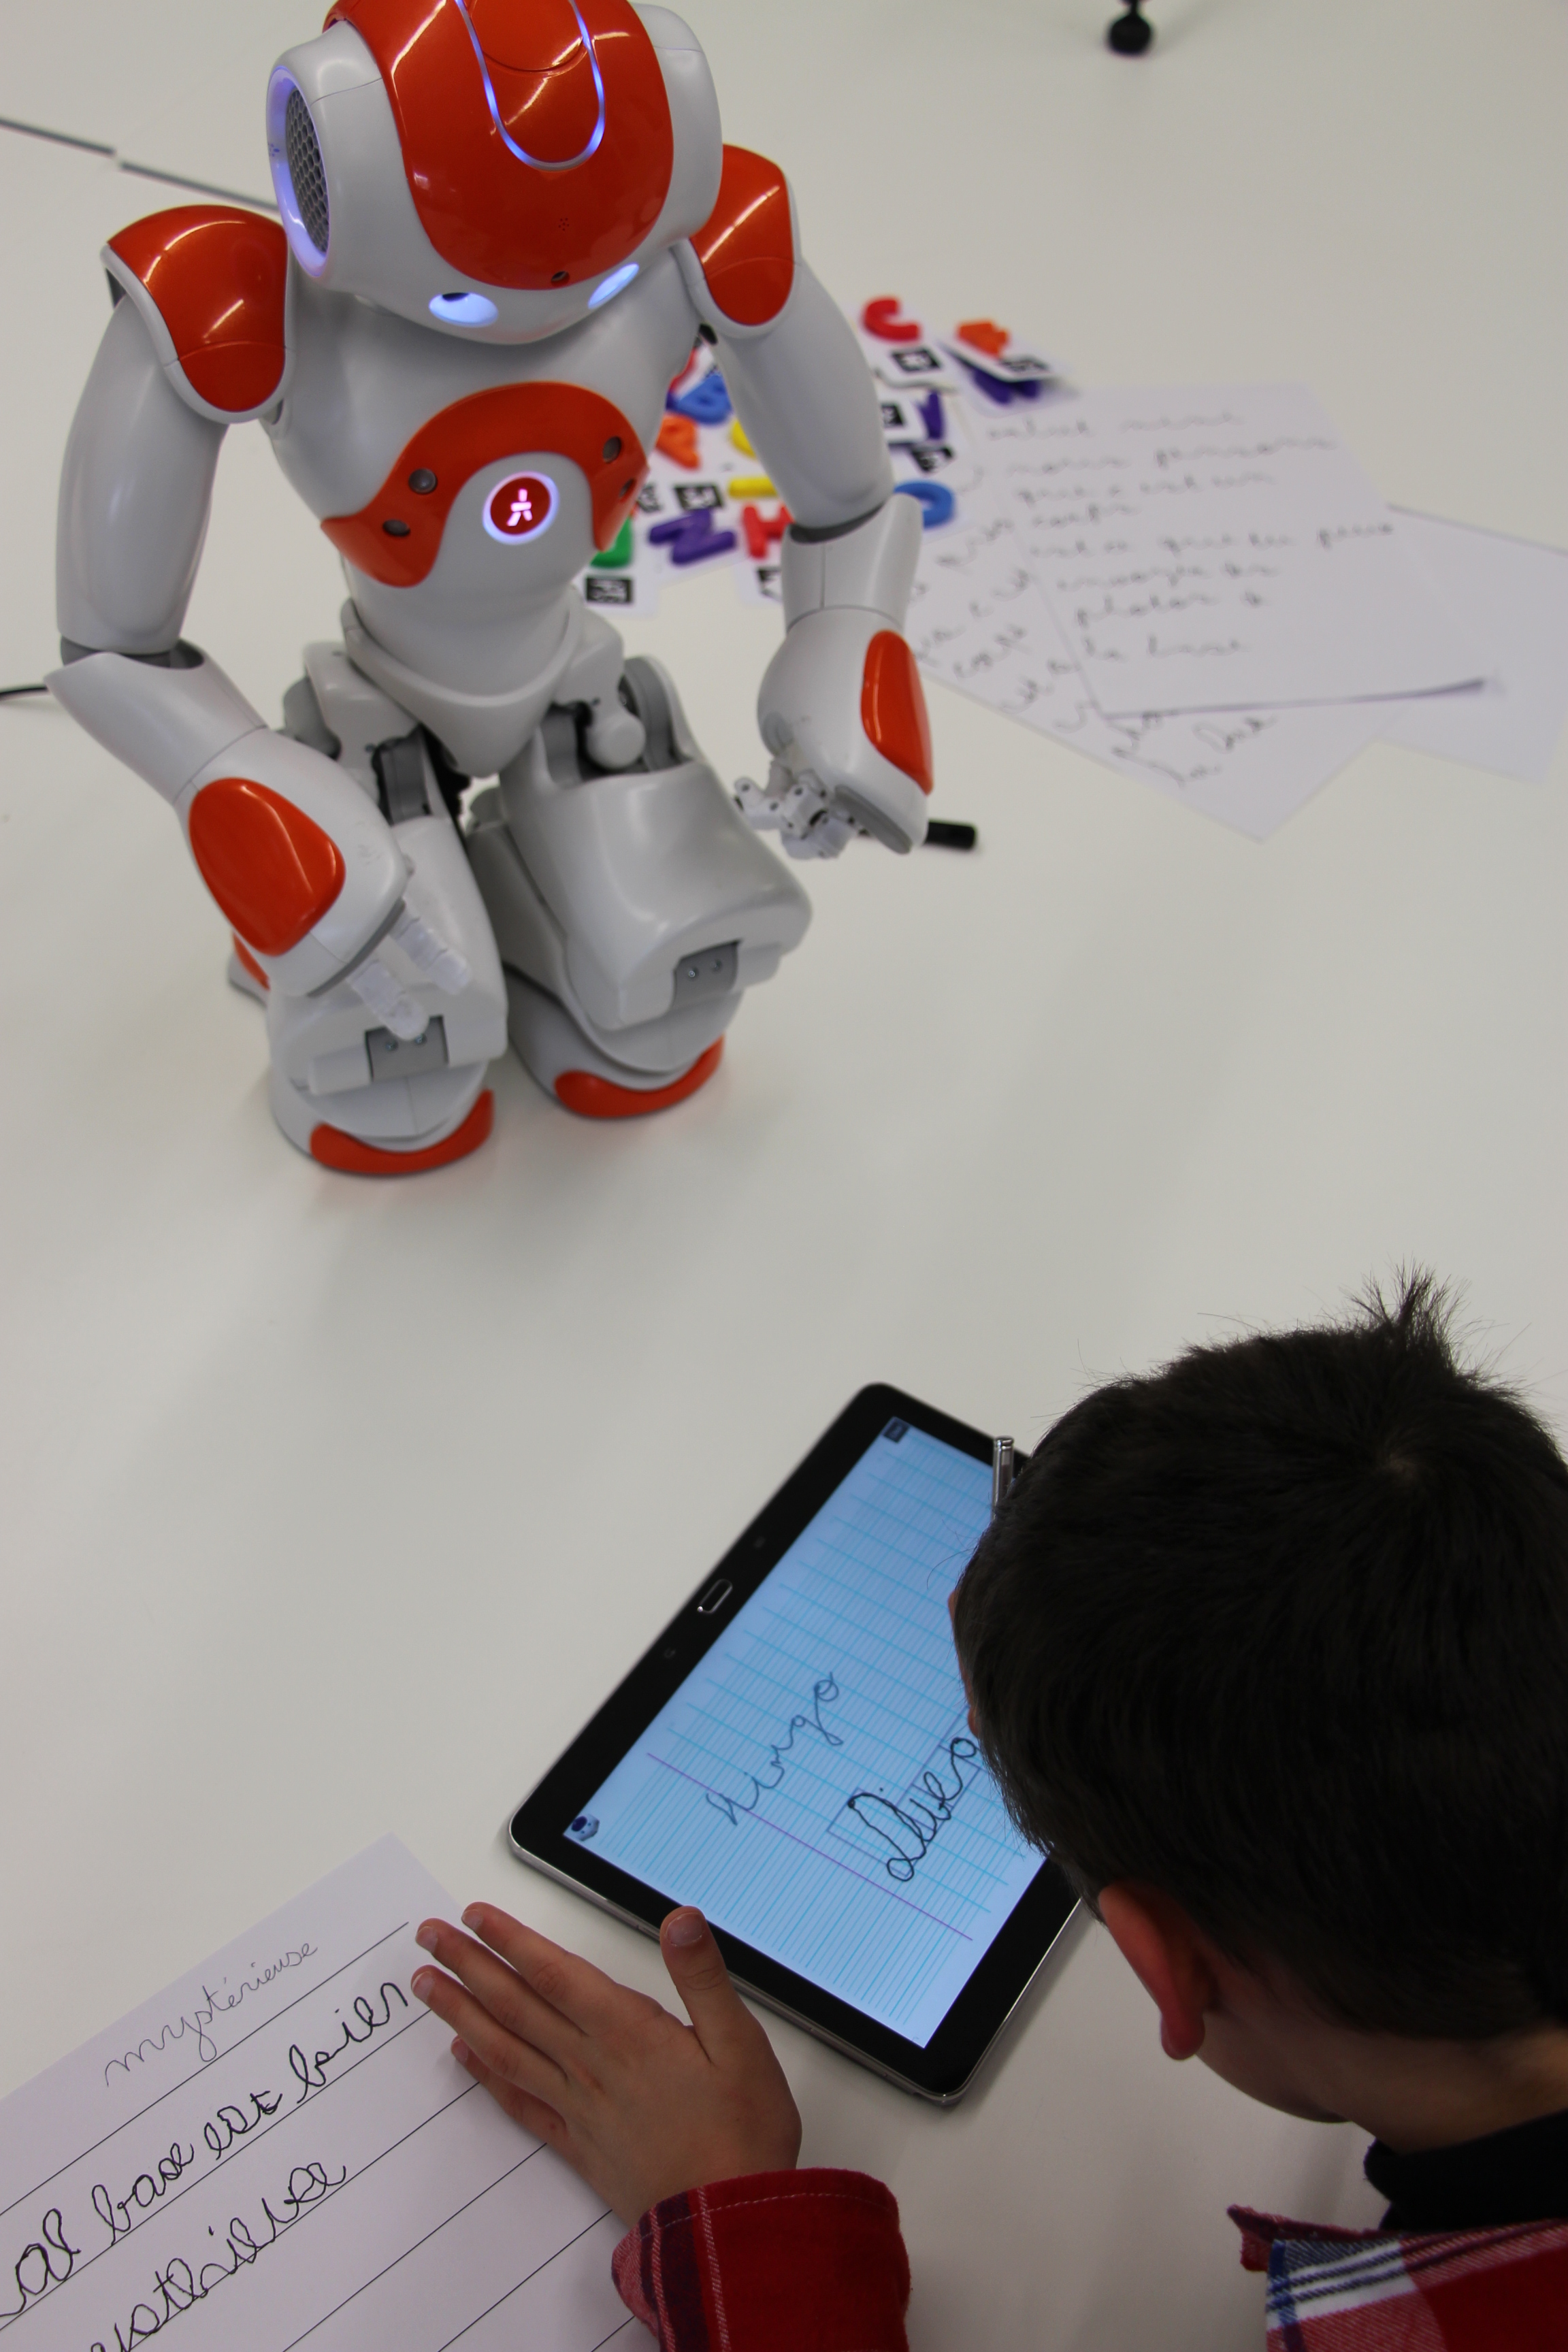
\includegraphics[width=0.8\linewidth]{cowriter/diego-correct}
            \end{center}
        \end{column}
        \begin{column}{0.5\linewidth}
            \begin{itemize}
                \item<+-> The robot as a \textbf{cognitive agent} is key here
                    \begin{itemize}
                        \item Protégé effect
                        \item metacognition
                    \end{itemize}
                \item<+-> A \textbf{social agent} for the child vs a
                    \textbf{tool} for the teacher!
            \end{itemize}
        \end{column}
    \end{columns}
\end{frame}

%%%%%%%%%%%%%%%%%%%%%%%%%%%%%%%%%%%%%%%%%%%%%%%%%%%%%%%%
%%%%%%%%%%%%%%%%%%%%%%%%%%%%%%%%%%%%%%%%%%%%%%%%%%%%%%%%
%%%%%%%%%%%%%%%%%%%%%%%%%%%%%%%%%%%%%%%%%%%%%%%%%%%%%%%%

\section{How hard is that?}

\imageframe{pr2-baby-1}
\imageframe{pr2-baby-2}
\imageframe{pr2-baby-3}
\imageframe{pr2-baby-4}


\begin{frame}{Taking the human perspective}

    \centering

    \begin{columns}
        \begin{column}{0.5\linewidth}
            How can the robot make sense of and act upon a command like:
            \vspace{2em}

            \bf
            ``Can you give me that book?''
        \end{column}
        \begin{column}{0.5\linewidth}
            \begin{center}
                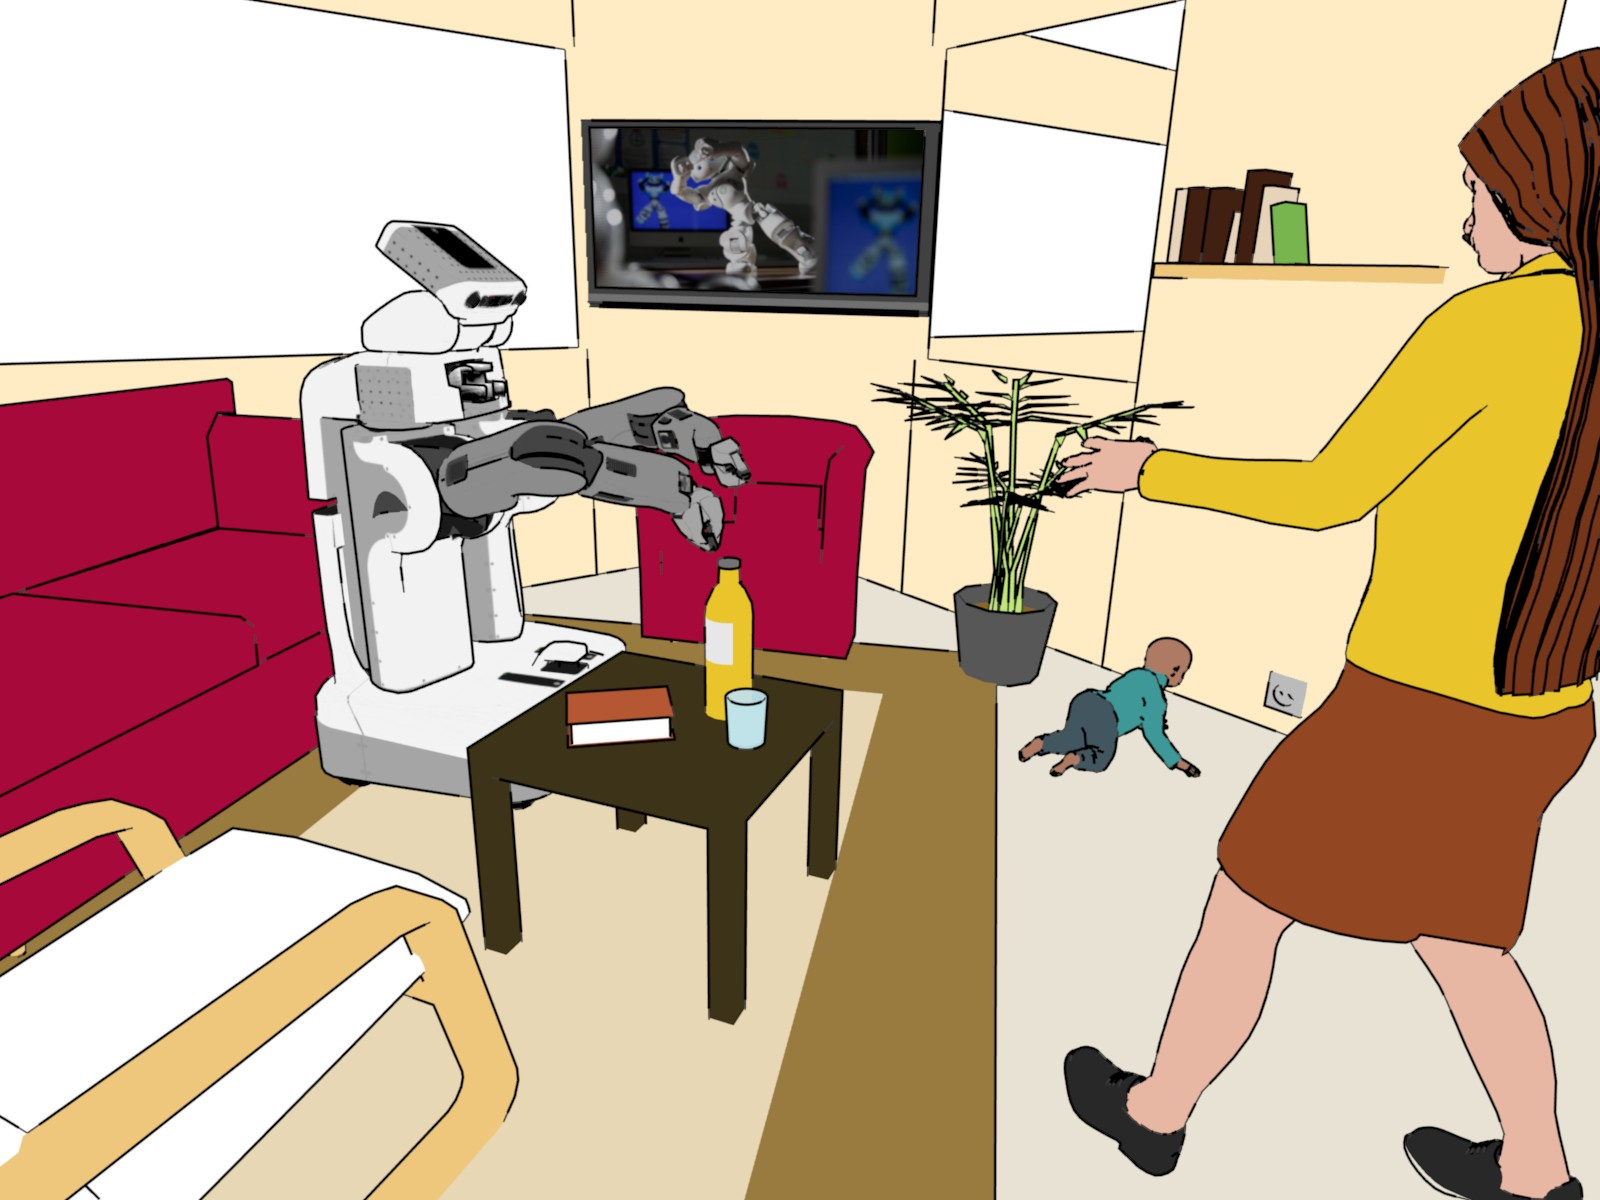
\includegraphics[width=\linewidth]{pr2-baby-3}
            \end{center}
        \end{column}
    \end{columns}

\end{frame}

\begin{frame}<3>{Multi-modal Symbolic situation assessment}

    \begin{columns}
        \begin{column}{0.4\linewidth}
        \centering
        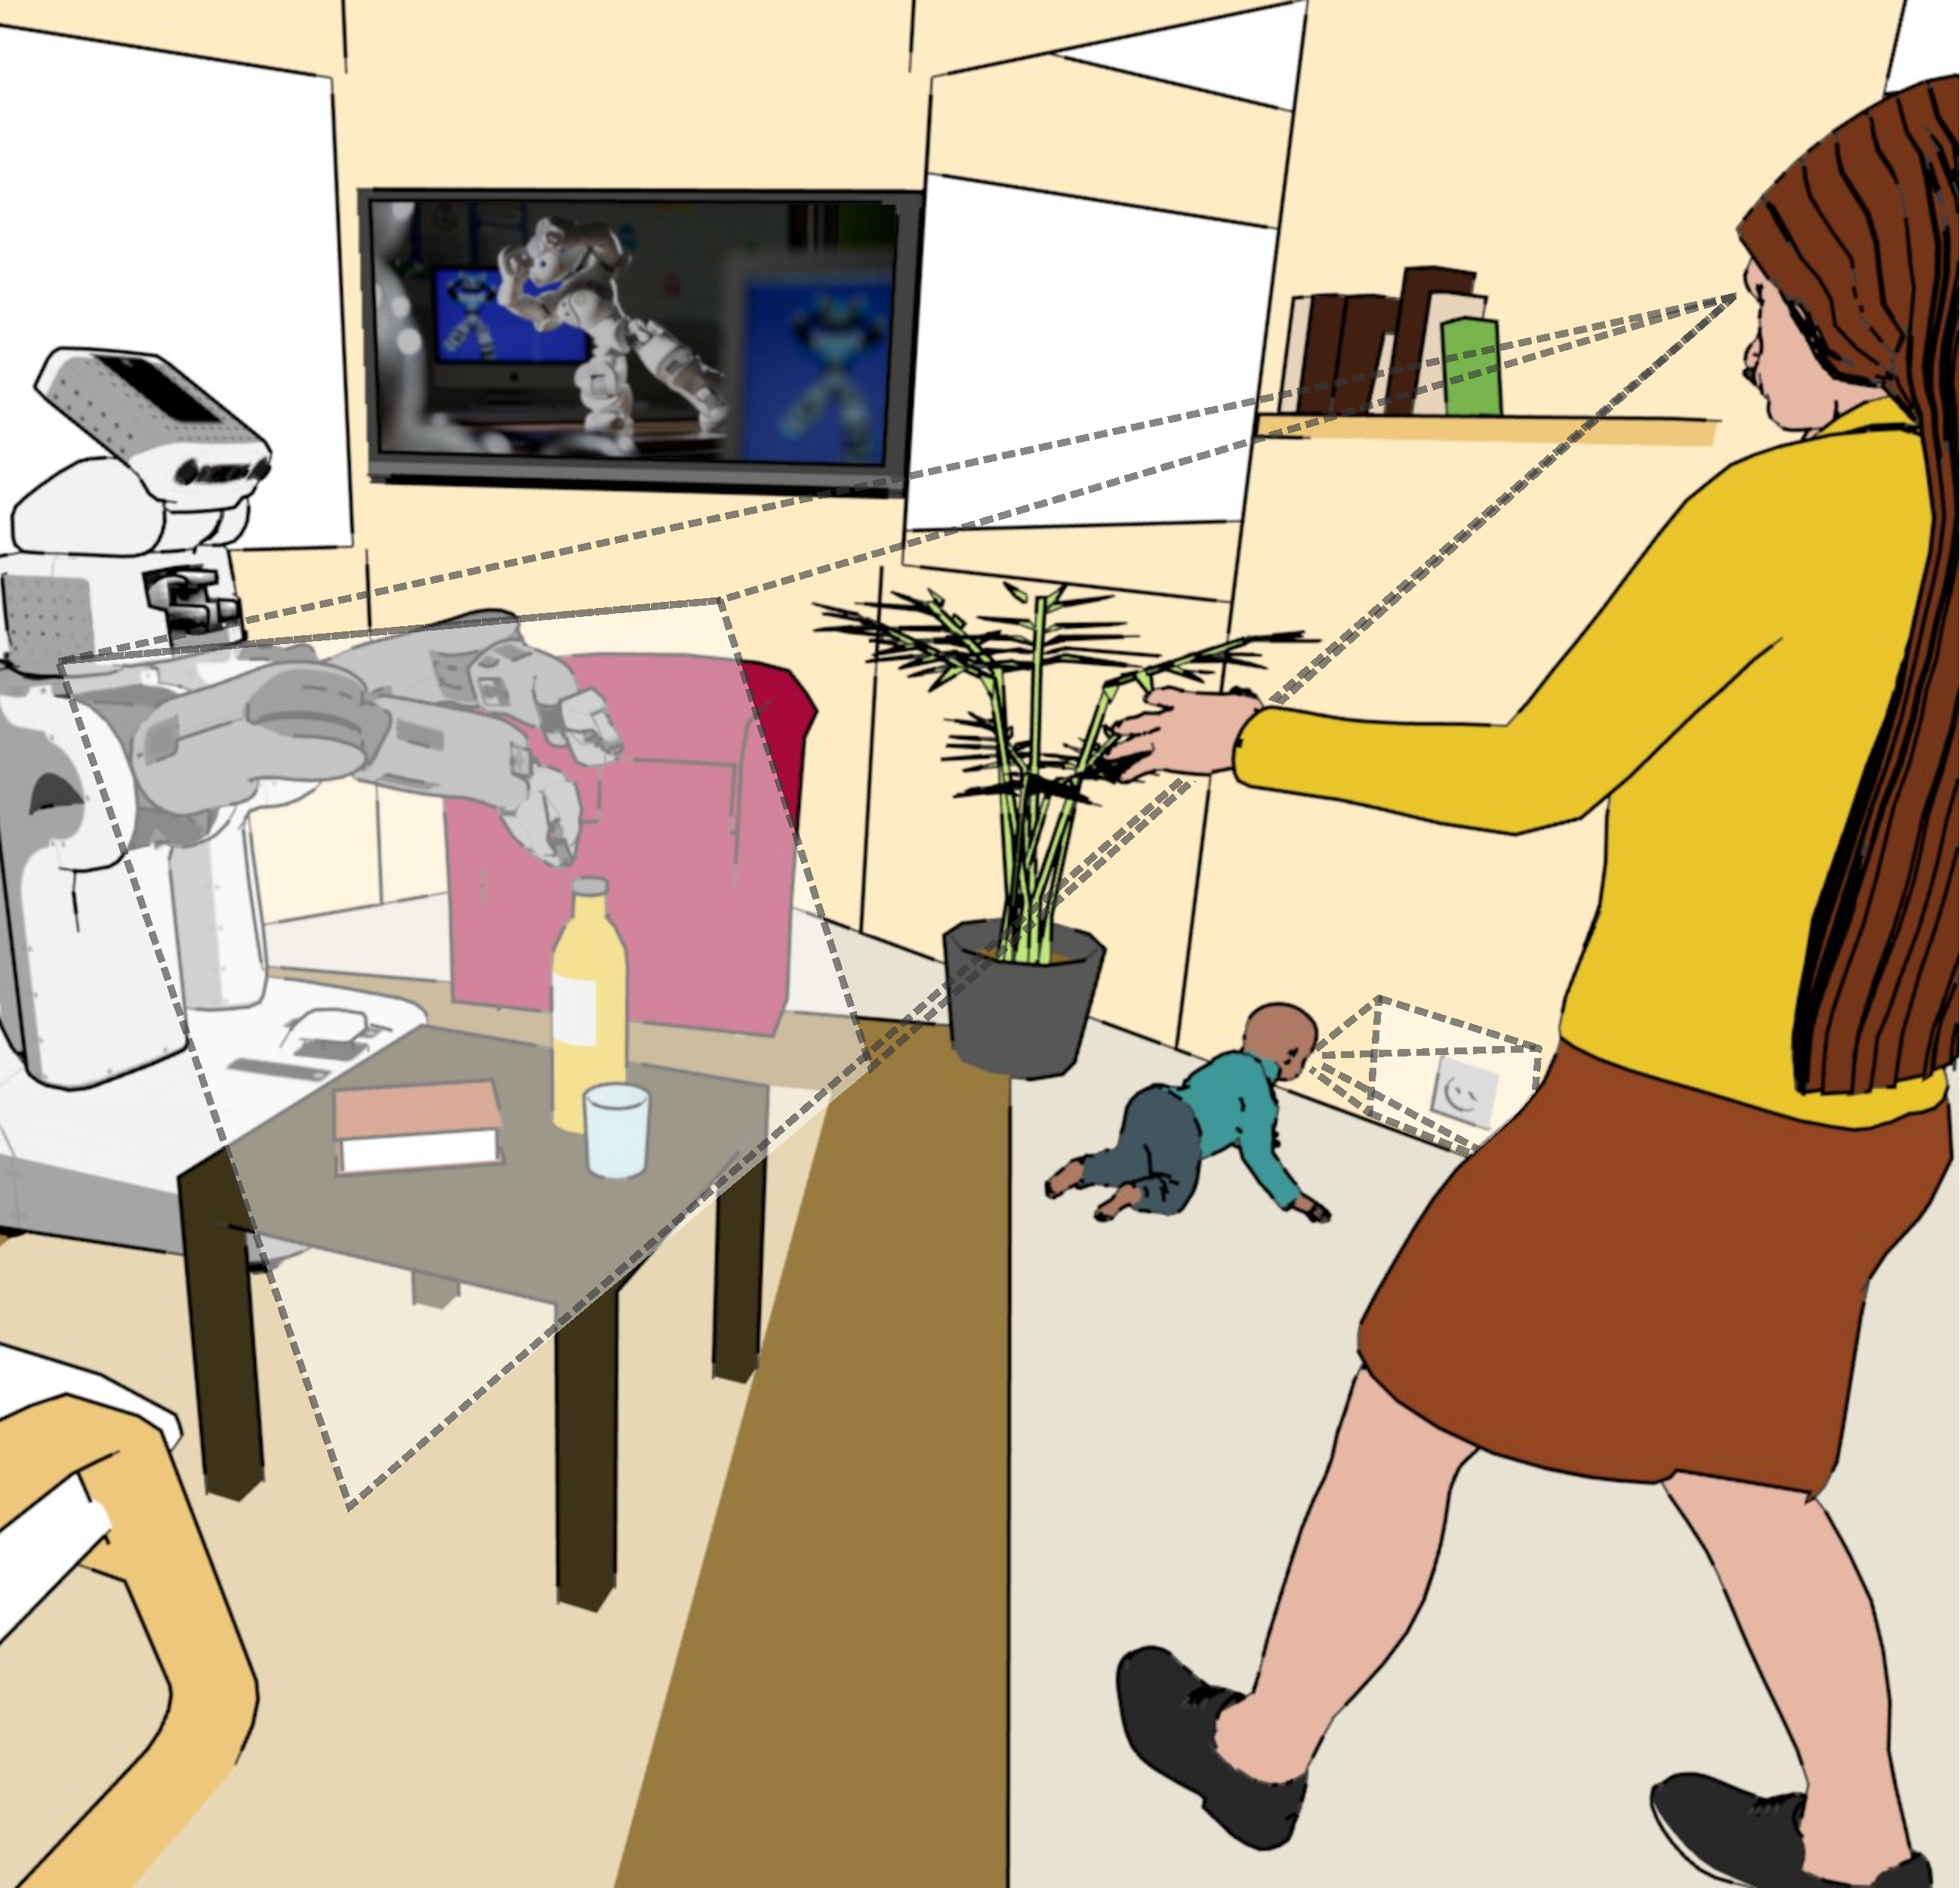
\includegraphics[width=\linewidth]{human-perspective-small}
             
        \end{column}
        \begin{column}{0.6\linewidth}
        
        \begin{figure}

        \resizebox{\columnwidth}{!}{%
        \begin{tikzpicture}[
            yscale=1.3,
            >=latex,
            every edge/.style={<-, draw, very thick},
            every node/.style={draw, font=\sf, node distance=0.5, rounded corners,
            align=center, inner sep=5pt,fill=hriSec2Dark!50},
            classof/.style={<-, draw=black!60, dashed},
            property/.style={<-, draw=hriSec2Comp},
            propname/.style={above, draw=none, fill=none, font=\tt, inner sep=2pt},
            instance/.style={draw=hriSec1Dark, font=\sf, node distance=0.5, rounded corners,
        align=center, inner sep=5pt, fill=none}]

            \node[fill=hriSec2Comp!50] (thing) {\textbf{thing}};
            \node [fill=hriSec3CompDark!50, node distance=1.8, below left=of
            thing](sthing) {place} edge[dashed] (thing);
            \node [fill=hriSec3CompDark!50, below left=of sthing] (agent) {agent} edge (sthing);
                \node [fill=hriSec3CompDark!50, below=of sthing] (artifact) {artifact} edge (sthing);
                \node [fill=hriSec3CompDark!50, below right=of sthing] (location) {physical
                support} edge (sthing);
                \node [fill=hriSec3CompDark!50, below right=of artifact] (table) {table}
                    edge (location) edge (artifact);


            \node [node distance=1, below right=of thing] (tthing) {temporal thing} edge (thing);
                \node [below right=of tthing] (evt) {event} edge[dashed] (tthing);
                            \node [below right=of evt] (act) {action} edge (evt);

        \uncover<2->{
        \draw[dotted, thick] (-8,-3.8) -- +(16, 0);

        \node [instance, below=3 of agent] (human) {human\_1} edge[classof, bend left] (agent);
        \node [instance, above left=of human] (human2) {human\_2} edge[classof, bend left] (agent);
        \node [instance, above right=of human, anchor=south] (robot) {myself} edge[classof, bend left] (agent);
        \node [instance, right=of human, anchor=north west] (book) {book\_game\_thrones}
        edge[classof] (artifact);
        \node [instance, right=2 of robot] (ikea) {ikea\_table} edge[classof, bend
        right] (table);
        \node [instance, right=2 of book] (brown) {brown} edge[property] node[propname] {hasColor} (book);


        }
        \uncover<3>{
        \draw[dotted, thick] (-8,-6.2) -- +(16, 0);

        \node [instance, below=5 of act] (moving) {move\_act\_42} edge[classof] (act);
        \path (moving.west) edge [property, out=180, in=-80, looseness=1] node[propname,below] {currentlyPerforms} (human.230);
        \path (book.250) edge [property, out=200, in=-80, looseness=1] node[propname,right]{looksAt} (human.280);
        \path (ikea.south) edge [property, out=-90, in=-80, looseness=2.5] node[propname, auto] {isOn} (book.320);
        }
        \end{tikzpicture}
        }

        \end{figure}

       \end{column}
    \end{columns}

\end{frame}

\begin{frame}{Dialogue Grounding}
    \centering

    \begin{columns}
        \begin{column}{0.65\linewidth}

    \centering
    \vspace*{2em}
    {\bf ``Give me that book''}\\

    \uncover<2-> {
        $\downarrow$\\
        {\tt me} $\rightarrow$ {\tt human\_1} \\
        find({\tt\scriptsize ?obj type Book, human\_1 focusesOn ?obj})
        $\rightarrow$ {\tt book\_game\_thrones} \\
    }

    \uncover<3-> {
        $\downarrow$\\
        { \tt
            \textbf{human\_1} desires \textbf{give\_act\_1}, \\
            \textbf{give\_act\_1} type \textbf{Give}, \\
            \textbf{give\_act\_1} performedBy \textbf{myself}, \\
            \textbf{give\_act\_1} actsOnObject \textbf{book\_GoT}, \\
            \textbf{give\_act\_1} receivedBy \textbf{human\_1} \\
        }
    }
            
        \end{column}
        \begin{column}{0.35\linewidth}
         \resizebox{\linewidth}{!}{%
 
 
             \begin{tikzpicture}[
                     >=latex,
                 every edge/.style={draw, very thick},
                 skill/.style={draw, rounded corners, align=center, inner sep=5pt, fill=black!20},
                 label/.style={midway, align=center, font=\scriptsize, above},
                 subpart/.style={rounded corners, draw, align=center, font=\scriptsize, fill opacity=0.5, text opacity=1, fill=white!50}]
 
             %%% PARSING
 
             \node at (0,0)[skill, fill=hriSec3CompDark!50] (prepro) {Pre-processing};
                 \node [left=0.7 of prepro] (input) {\textbf{Input}};
                 \path (input) edge [->] (prepro);
 
                 %\path (spark.100) edge [->, bend right] node[label] {symbolic \\ facts} (oro);
                 \node [below =0.4 of prepro, skill, fill=hriSec3CompDark!50] (parsing) {Parsing};
                 \path (prepro) edge [->] (parsing);
 
                 \coordinate (base-onto) at (4,0);
 
                 %%% RESOLUTION
                     \node [below=0.4 of parsing, skill, fill=hriSec3!50, minimum height=4cm, minimum width=5cm] (resolution) {};
                 \node [subpart, below=0.2 of resolution.115] (pron) {Pronouns \& \\ anaphora resolution};
                 \node [subpart, below=0.2 of pron] (noun) {Noun phrase \\ resolution};
                 \node [subpart, right=0.3 of noun, anchor=north west] (discr) {Discrimination};
                 \node [subpart, below=0.2 of noun] (verb) {Verbal phrase \\ resolution};
                 \node [subpart, cylinder, shape border rotate=90, aspect=0.5, below=0.2 of discr] (actions) {Actions};
                 \path (pron) edge [->] (noun);
                 \path (noun) edge [->] (discr);
                 \path (noun) edge [->] (verb);
                 \path (verb) edge [dashed, <->] (actions);
                 \path (pron) edge [dashed, <->] node[label] {queries} (pron -| base-onto);
                 \path (noun.20) edge [dashed, <->] node[label] {queries} (noun.20 -| base-onto);
                 \path (discr) edge [<->] (discr -| base-onto);
 
                 \node [left=0.2 of resolution.west, rotate=90, anchor=south] {Resolution};
                 \path (parsing) edge [->] (pron);
 
             %%% INTERPRETATION
                     \node [skill, below=0.4 of resolution,minimum width=5cm, minimum height=3cm] (interp) {};
                 \node [subpart, below=0.2 of interp.north] (content) {Content analysis};
                 \node [below=0.6 of content.south west, subpart] (question) {Question \\ handler};
                 \node [below=0.6 of content.south east, subpart] (stat) {Statement \\ builder};
                 \path (content) edge [->] node[label, left] {question} (question);
                 \path (content) edge [->] node [label, right] {goal | statement} (stat);
                 \path (stat) edge [->] node [label] {asserts} (stat -| base-onto);
 
                 \node [left=0.2 of interp.west, rotate=90, anchor=south] {Interpretation};
 
                 \path (verb) edge [->] (content);
                 \path (question) edge [dashed, bend right, <->] node[label] {queries} (question.south -| base-onto);
 
             %%% ONTOLOGY
                     \node at (resolution.north -| base-onto) [rotate=-90, skill, minimum height=2cm, minimum width=7cm, fill=hriSec3!50, anchor=south west] (onto) {Ontology server};
 
 
             %%% VERBALIZATION
                 \node [below=0.7 of interp, skill, fill=hriSec2Dark!50] (verb) {Verbalization};
             \path (question) edge [->] (verb);
             \path (stat) edge [->] (verb);
             \path (discr.south east) edge [black!50, dashed, bend left, <->] (verb.north east);
             \node [right=0.7 of verb] (output) {\textbf{Output}};
             \path (verb) edge [->] (output);
         \end{tikzpicture}
         }

        \end{column}
    \end{columns}

\end{frame}

%\begin{frame}[fragile]{Finally, add a controller}
%\begin{pythoncode}
%
%
%import kb # pip install pykb
%kb = kb.KB()
%
%kb.subscribe(["HUMAN desires ?action"], onDesire)
%
%def onDesire(desire):
%        print("The human wants something!")
%        action = kb[desire + " rdf:type ?type"]
%        object = kb[desire + " actsOnObject ?object"]
%
%        if action == "Give":
%            robot.give(object) # <-- up to you!!
%
%        if action == "Get":
%            place = kb[object + " isAt ?place"] # isOn, isIn...
%            robot.goto(place) # <-- up to you!
%            robot.pick(object) # <-- up to you!
%
%\end{pythoncode}
%\end{frame}

\videoframe[0.56]{figs/this_box.avi}
%\videoframe[0.56]{figs/this_box.webm?autostart&start=1}


%\begin{frame}[fragile]
%\begin{pythoncode}
%    from robots import GenericRobot
%    from robots.concurrency import action, ActionCancelled
%    from robots.resources import Resource, lock
%
%    class MyRobot(GenericRobot):
%        # ... state + lowlevel action
%
%    WHEELS = Resource("wheels")
%
%    @lock(WHEELS)
%    @action
%    def move_forward(robot):
%        target = [1.0, 0., 0., "base_link"]
%
%        try:
%            robot.goto(target)
%
%            while(robot.dist_to(target) > 0.1):
%                robot.sleep(0.5)
%
%        except ActionCancelled:
%            robot.stop()
%
%\end{pythoncode}
%\end{frame}
%
%%%%%%%%%%%%%%%%%%%%%%%%%%%%%%%%%%%%%%%%%%%%%%%%%%%%%%%%%
%
%\begin{frame}[fragile]
%\begin{pythoncode}
%    with MyRobot() as robot:
%
%        robot.whenever("my_bumper", True).do(move_forward)
%
%        try:
%            while True:
%                time.sleep(0.5)
%        except KeyboardInterrupt:
%            pass
%\end{pythoncode}
%\end{frame}


\section{A pinch of social psychology:\\false beliefs!}


\begin{frame}[plain]

    \begin{center}
        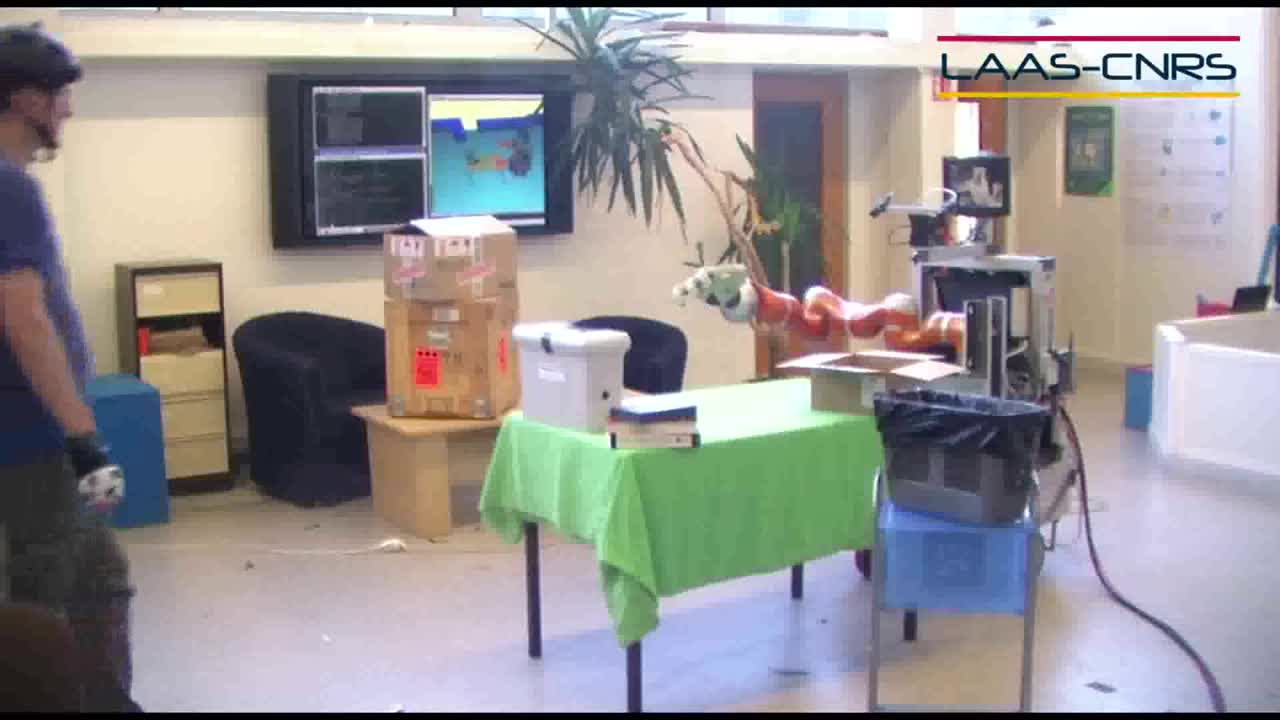
\includegraphics[width=0.8\linewidth]{figs/this_box_thumb}

        What if I ask for the video tape in the box, but the robot previously
        moved it somewhere else?


    \end{center}
\end{frame}

\imageframe[scale=0.9]{sally_ann}

\begin{frame}{Just clone it!}
        \begin{multicols}{2}
            \begin{figure}
                \resizebox{0.4\textwidth}{!}{
                    \begin{tikzpicture}[
                        >=latex,
                        every edge/.style={<-, draw, very thick},
                        every node/.style={draw, font=\sf, node distance=0.5, rounded corners,
                                        align=center, inner sep=5pt,fill=hriSec2Dark!50},
                        classof/.style={<-, draw=black!60, dashed},
                        property/.style={<-, draw=hriSec2Comp},
                        propname/.style={above, draw=none, fill=none, font=\tt, inner sep=2pt},
                        instance/.style={draw=hriSec1Dark, font=\sf, node distance=0.5, rounded corners,
                        align=center, inner sep=5pt, fill=white}]

                    \node[fill=hriSec2Comp!50] (thing) {\textbf{thing}};
                    \node [fill=hriSec3CompDark!50, node distance=1.8, below left=of thing](sthing) {place} edge[dashed] (thing);
                    \node [fill=hriSec3CompDark!50, below left=of sthing] (agent) {agent} edge (sthing);
                        \node [fill=hriSec3CompDark!50, below=of sthing] (artifact) {artifact} edge (sthing);
                        \node [fill=hriSec3CompDark!50, below right=of sthing] (location) {physical
                        support} edge (sthing);
                        \node [fill=hriSec3CompDark!50, below right=of artifact] (table) {table}
                            edge (location) edge (artifact);


                    \node [node distance=1, below right=of thing] (tthing) {temporal thing} edge (thing);
                        \node [below right=of tthing] (evt) {event} edge[dashed] (tthing);
                                    \node [below right=of evt] (act) {action} edge (evt);

                \draw[dotted, thick] (-7,-5) -- (7.5, -5);

                \node [instance, below=3 of agent] (human) {human\_1} edge[classof, bend left] (agent);
                \node [instance, above left=of human] (human2) {human\_2} edge[classof, bend left] (agent);
                \node [instance, above right=of human, anchor=south] (robot) {pr2\_robot} edge[classof, bend left] (agent);
;
                \node [instance, right=of human, anchor=north west] (book) {book\_game\_thrones}
                edge[classof] (artifact);
                \node [instance, right=3 of robot] (ikea) {ikea\_table} edge[classof, bend
                right] (table);
                \node [instance, right=2 of book] (red) {red} edge[property] node[propname] {hasColor} (book);

                \node [instance,right=1 of robot,fill=hriSec2] {myself} edge[property] node[propname, auto,above] {$\equiv$} (robot);

                \draw[dotted, thick] (-7,-8) -- (7.5, -8);

                \path (book.200) edge [property, out=-100, in=-80, looseness=2]
                node[propname,auto] {isNextTo} (human.south);
                \path (book.270) edge [property, out=-100, in=-90, looseness=3.5] node[propname,auto] {looksAt} (robot.south);
                \path (ikea.south) edge [property, out=-90, in=-80, looseness=3] node[propname, auto] {isOn} (book.320);
                \end{tikzpicture}
            }

            \end{figure}
            \begin{figure}
                \resizebox{0.4\textwidth}{!}{
                    \begin{tikzpicture}[
                        >=latex,
                        every edge/.style={<-, draw, very thick},
                        every node/.style={draw, font=\sf, node distance=0.5, rounded corners,
                                        align=center, inner sep=5pt,fill=hriSec2Dark!50},
                        classof/.style={<-, draw=black!60, dashed},
                        property/.style={<-, draw=hriSec2Comp},
                        propname/.style={above, draw=none, fill=none, font=\tt, inner sep=2pt},
                        instance/.style={draw=hriSec1Dark, font=\sf, node distance=0.5, rounded corners,
                        align=center, inner sep=5pt, fill=white}]

                    \node[fill=hriSec2Comp!50] (thing) {\textbf{thing}};
                    \node [fill=hriSec3CompDark!50, node distance=1.8, below left=of thing](sthing) {place} edge[dashed] (thing);
                    \node [fill=hriSec3CompDark!50, below left=of sthing] (agent) {agent} edge (sthing);
                        \node [fill=hriSec3CompDark!50, below=of sthing] (artifact) {artifact} edge (sthing);
                        \node [fill=hriSec3CompDark!50, below right=of sthing] (location) {physical
                        support} edge (sthing);
                        \node [fill=hriSec3CompDark!50, below right=of artifact] (table) {table}
                            edge (location) edge (artifact);


                    \node [node distance=1, below right=of thing] (tthing) {temporal thing} edge (thing);
                        \node [below right=of tthing] (evt) {event} edge[dashed] (tthing);
                                    \node [below right=of evt] (act) {action} edge (evt);

                \draw[dotted, thick] (-7,-5) -- (7.5, -5);

                \node [instance, below=3 of agent] (human) {human\_1} edge[classof, bend left] (agent);
                \node [instance, above left=of human] (human2) {human\_2} edge[classof, bend left] (agent);
                \node [instance, above right=of human, anchor=south] (robot) {pr2\_robot} edge[classof, bend left] (agent);
;
                \node [instance, right=of human, anchor=north west] (book) {book\_game\_thrones}
                edge[classof] (artifact);
                \node [instance, right=3 of robot] (ikea) {ikea\_table} edge[classof, bend
                right] (table);
                \node [instance, right=2 of book] (red) {red} edge[property] node[propname] {hasColor} (book);

                \node [instance,below left=1 of human,fill=hriSec2] {myself} edge[property] node[propname, auto,above] {$\equiv$} (human);

                \draw[dotted, thick] (-7,-8) -- (7.5, -8);

                \path (book.200) edge [property, out=-100, in=-80, looseness=2]
                node[propname,auto] {isNextTo} (human.south);
                \path (book.270) edge [property, out=-100, in=-90, looseness=3.5] node[propname,auto] {looksAt} (robot.south);
                \path (ikea.south) edge [property, out=-90, in=-80, looseness=3] node[propname, auto] {isOn} (book.320);
                \end{tikzpicture}
            }
            \end{figure}
            \begin{figure}
                \resizebox{0.4\textwidth}{!}{
                    \begin{tikzpicture}[
                        >=latex,
                        every edge/.style={<-, draw, very thick},
                        every node/.style={draw, font=\sf, node distance=0.5, rounded corners,
                                        align=center, inner sep=5pt,fill=hriSec2Dark!50},
                        classof/.style={<-, draw=black!60, dashed},
                        property/.style={<-, draw=hriSec2Comp},
                        propname/.style={above, draw=none, fill=none, font=\tt, inner sep=2pt},
                        instance/.style={draw=hriSec1Dark, font=\sf, node distance=0.5, rounded corners,
                        align=center, inner sep=5pt, fill=white}]

                    \node[fill=hriSec2Comp!50] (thing) {\textbf{thing}};
                    \node [fill=hriSec3CompDark!50, node distance=1.8, below left=of thing](sthing) {place} edge[dashed] (thing);
                    \node [fill=hriSec3CompDark!50, below left=of sthing] (agent) {agent} edge (sthing);
                        \node [fill=hriSec3CompDark!50, below=of sthing] (artifact) {artifact} edge (sthing);
                        \node [fill=hriSec3CompDark!50, below right=of sthing] (location) {physical
                        support} edge (sthing);
                        \node [fill=hriSec3CompDark!50, below right=of artifact] (table) {table}
                            edge (location) edge (artifact);


                    \node [node distance=1, below right=of thing] (tthing) {temporal thing} edge (thing);
                        \node [below right=of tthing] (evt) {event} edge[dashed] (tthing);
                                    \node [below right=of evt] (act) {action} edge (evt);

                \draw[dotted, thick] (-7,-5) -- (7.5, -5);

                \node [instance, below=3 of agent] (human) {human\_1} edge[classof, bend left] (agent);
                \node [instance, above left=of human] (human2) {human\_2} edge[classof, bend left] (agent);
                \node [instance, above right=of human, anchor=south] (robot) {pr2\_robot} edge[classof, bend left] (agent);
;
                \node [instance, right=of human, anchor=north west] (book) {book\_game\_thrones}
                edge[classof] (artifact);
                \node [instance, right=3 of robot] (ikea) {ikea\_table} edge[classof, bend
                right] (table);
                \node [instance, right=2 of book] (red) {red} edge[property] node[propname] {hasColor} (book);

                \node [instance,below=1 of human2,fill=hriSec2] {myself} edge[property] node[propname, auto] {$\equiv$} (human2);

                \draw[dotted, thick] (-7,-8) -- (7.5, -8);

                \path (book.200) edge [property, out=-100, in=-80, looseness=2]
                node[propname,auto] {isNextTo} (human.south);
                \path (book.270) edge [property, out=-100, in=-90, looseness=3.5] node[propname,auto] {looksAt} (robot.south);
                \path (ikea.south) edge [property, out=-90, in=-80, looseness=3] node[propname, auto] {isOn} (book.320);
                \end{tikzpicture}
            }
            \end{figure}
            {\vspace*{1.5cm}\hspace*{2.5cm}\huge...}
        \end{multicols}
\end{frame}

\section{Project ideas}


\imageframe[color=black]{cozmo-expression-sheet}
\videoframe[0.56]{figs/pinsoro-matplotlib.mp4}
\imageframe[color=black]{tiago}
\videoframe[0.56]{figs/underworlds.avi?start=20}

\begin{frame}[plain]


    \Huge
    \textbf{Sounds good?}

    \large

    \vspace{2em}
    Bring in your ideas!\\

    severin.lemaignan@brl.ac.uk \\
    (or Manuel, or Praminda!)

\end{frame}


{
    \fullbackground[color=black]{trump}

\begin{frame}[plain]

    \color{white}

    \Huge
    \textbf{I like this guy!}

    \vfill

\end{frame}
}


\end{document}






